\documentclass{standalone}
\usepackage{tikz}
\usetikzlibrary{patterns}
\usetikzlibrary{positioning}
\usetikzlibrary{patterns, positioning}
\usetikzlibrary{shapes.misc}
\usepackage[outline]{contour}
\contourlength{1.5pt} 
\usepackage[sfdefault]{ClearSans}

\begin{document}
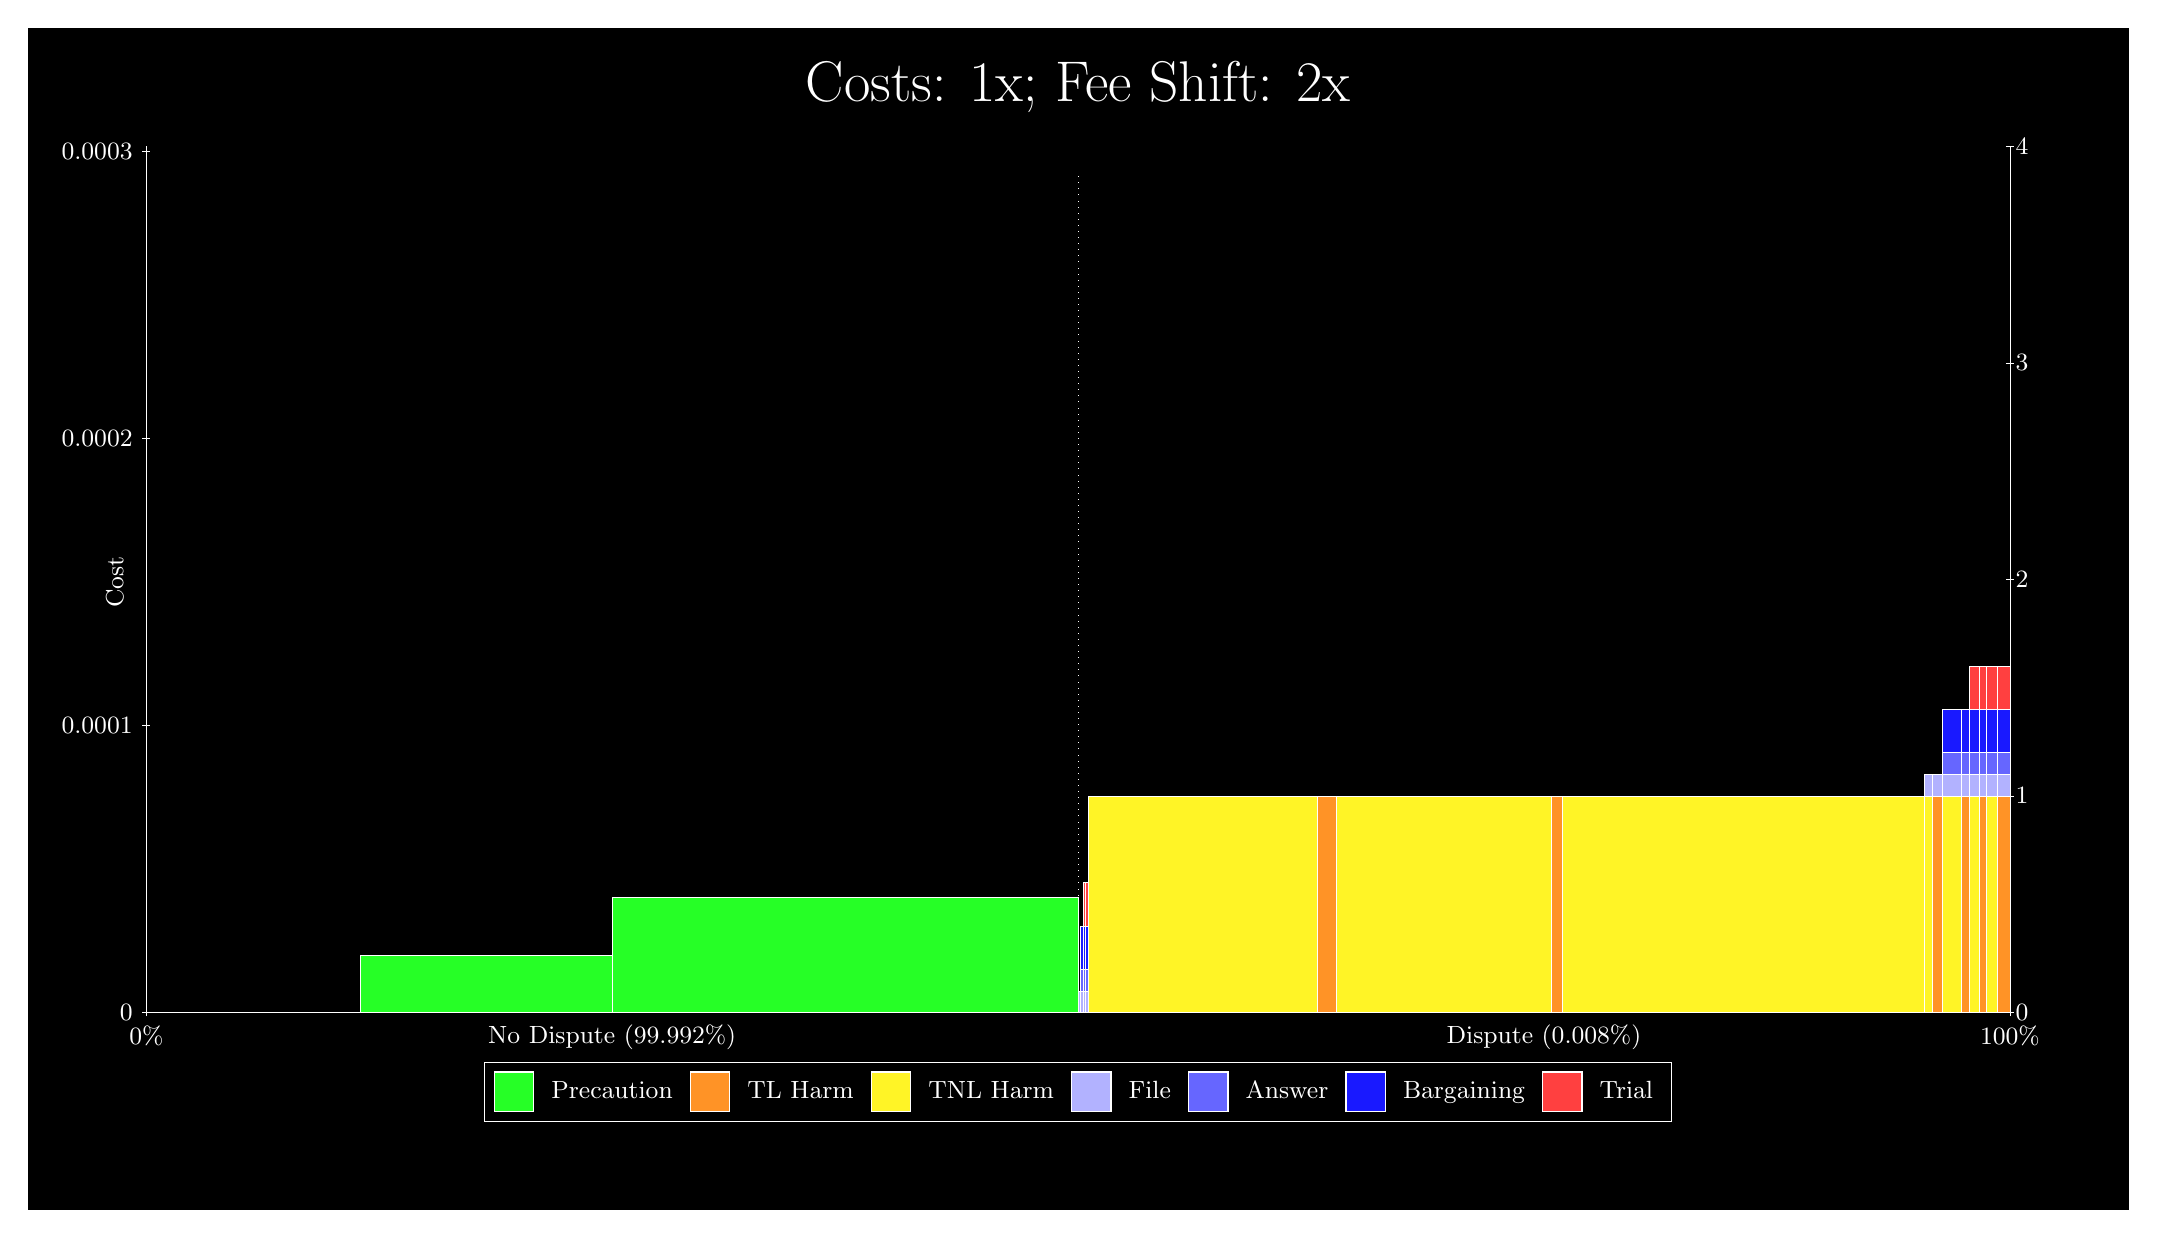
\begin{tikzpicture}
\draw[fill=black] (0,0) rectangle (26.667,15);
\draw[draw=none,text=white] (0,13.5) rectangle (26.667,15) node[midway] {\huge Costs: 1x; Fee Shift: 2x };
\draw[fill=green!85,draw=white,very thin] (4.2218,2.5) rectangle (7.4166,3.2292);
\draw[fill=green!85,draw=white,very thin] (7.4166,2.5) rectangle (13.333,3.9584);
\draw[fill=blue!30,draw=white,very thin] (13.333,2.5) rectangle (13.357,2.775);
\draw[fill=green!85,draw=white,very thin] (13.357,2.5) rectangle (13.399,2.5001);
\draw[fill=blue!30,draw=white,very thin] (13.357,2.5001) rectangle (13.399,2.7751);
\draw[fill=blue!60,draw=white,very thin] (13.357,2.7751) rectangle (13.399,3.0501);
\draw[fill=blue!90,draw=white,very thin] (13.357,3.0501) rectangle (13.399,3.6001);
\draw[fill=blue!30,draw=white,very thin] (13.399,2.5) rectangle (13.421,2.775);
\draw[fill=blue!60,draw=white,very thin] (13.399,2.775) rectangle (13.421,3.05);
\draw[fill=blue!90,draw=white,very thin] (13.399,3.05) rectangle (13.421,3.6);
\draw[fill=red!75,draw=white,very thin] (13.399,3.6) rectangle (13.421,4.15);
\draw[fill=green!85,draw=white,very thin] (13.421,2.5) rectangle (13.46,2.5001);
\draw[fill=blue!30,draw=white,very thin] (13.421,2.5001) rectangle (13.46,2.7751);
\draw[fill=blue!60,draw=white,very thin] (13.421,2.7751) rectangle (13.46,3.0501);
\draw[fill=blue!90,draw=white,very thin] (13.421,3.0501) rectangle (13.46,3.6001);
\draw[fill=red!75,draw=white,very thin] (13.421,3.6001) rectangle (13.46,4.1501);
\draw[fill=yellow!85,draw=white,very thin] (13.46,2.5) rectangle (16.369,5.25);
\draw[fill=orange!85,draw=white,very thin] (16.369,2.5) rectangle (16.616,5.25);
\draw[fill=green!85,draw=white,very thin] (16.616,2.5) rectangle (19.348,2.5001);
\draw[fill=yellow!85,draw=white,very thin] (16.616,2.5001) rectangle (19.348,5.2501);
\draw[fill=green!85,draw=white,very thin] (19.348,2.5) rectangle (19.477,2.5001);
\draw[fill=orange!85,draw=white,very thin] (19.348,2.5001) rectangle (19.477,5.2501);
\draw[fill=green!85,draw=white,very thin] (19.477,2.5) rectangle (24.075,2.5001);
\draw[fill=yellow!85,draw=white,very thin] (19.477,2.5001) rectangle (24.075,5.2501);
\draw[fill=yellow!85,draw=white,very thin] (24.075,2.5) rectangle (24.181,5.25);
\draw[fill=blue!30,draw=white,very thin] (24.075,5.25) rectangle (24.181,5.525);
\draw[fill=orange!85,draw=white,very thin] (24.181,2.5) rectangle (24.314,5.25);
\draw[fill=blue!30,draw=white,very thin] (24.181,5.25) rectangle (24.314,5.525);
\draw[fill=green!85,draw=white,very thin] (24.314,2.5) rectangle (24.551,2.5001);
\draw[fill=yellow!85,draw=white,very thin] (24.314,2.5001) rectangle (24.551,5.2501);
\draw[fill=blue!30,draw=white,very thin] (24.314,5.2501) rectangle (24.551,5.5251);
\draw[fill=blue!60,draw=white,very thin] (24.314,5.5251) rectangle (24.551,5.8001);
\draw[fill=blue!90,draw=white,very thin] (24.314,5.8001) rectangle (24.551,6.3501);
\draw[fill=green!85,draw=white,very thin] (24.551,2.5) rectangle (24.649,2.5001);
\draw[fill=orange!85,draw=white,very thin] (24.551,2.5001) rectangle (24.649,5.2501);
\draw[fill=blue!30,draw=white,very thin] (24.551,5.2501) rectangle (24.649,5.5251);
\draw[fill=blue!60,draw=white,very thin] (24.551,5.5251) rectangle (24.649,5.8001);
\draw[fill=blue!90,draw=white,very thin] (24.551,5.8001) rectangle (24.649,6.3501);
\draw[fill=yellow!85,draw=white,very thin] (24.649,2.5) rectangle (24.775,5.25);
\draw[fill=blue!30,draw=white,very thin] (24.649,5.25) rectangle (24.775,5.525);
\draw[fill=blue!60,draw=white,very thin] (24.649,5.525) rectangle (24.775,5.8);
\draw[fill=blue!90,draw=white,very thin] (24.649,5.8) rectangle (24.775,6.35);
\draw[fill=red!75,draw=white,very thin] (24.649,6.35) rectangle (24.775,6.9);
\draw[fill=orange!85,draw=white,very thin] (24.775,2.5) rectangle (24.864,5.25);
\draw[fill=blue!30,draw=white,very thin] (24.775,5.25) rectangle (24.864,5.525);
\draw[fill=blue!60,draw=white,very thin] (24.775,5.525) rectangle (24.864,5.8);
\draw[fill=blue!90,draw=white,very thin] (24.775,5.8) rectangle (24.864,6.35);
\draw[fill=red!75,draw=white,very thin] (24.775,6.35) rectangle (24.864,6.9);
\draw[fill=green!85,draw=white,very thin] (24.864,2.5) rectangle (25.001,2.5001);
\draw[fill=yellow!85,draw=white,very thin] (24.864,2.5001) rectangle (25.001,5.2501);
\draw[fill=blue!30,draw=white,very thin] (24.864,5.2501) rectangle (25.001,5.5251);
\draw[fill=blue!60,draw=white,very thin] (24.864,5.5251) rectangle (25.001,5.8001);
\draw[fill=blue!90,draw=white,very thin] (24.864,5.8001) rectangle (25.001,6.3501);
\draw[fill=red!75,draw=white,very thin] (24.864,6.3501) rectangle (25.001,6.9001);
\draw[fill=green!85,draw=white,very thin] (25.001,2.5) rectangle (25.167,2.5001);
\draw[fill=orange!85,draw=white,very thin] (25.001,2.5001) rectangle (25.167,5.2501);
\draw[fill=blue!30,draw=white,very thin] (25.001,5.2501) rectangle (25.167,5.5251);
\draw[fill=blue!60,draw=white,very thin] (25.001,5.5251) rectangle (25.167,5.8001);
\draw[fill=blue!90,draw=white,very thin] (25.001,5.8001) rectangle (25.167,6.3501);
\draw[fill=red!75,draw=white,very thin] (25.001,6.3501) rectangle (25.167,6.9001);
\draw[white,very thin] (1.5,2.5) -- (1.5,13.5);
\node[font=\small,rotate=90,text=white, anchor=center] at (1.1, 7.9692) {Cost};
\draw[white,very thin] (1.45,2.5) -- (1.55,2.5);
\node[font=\small,text=white, anchor=east] at (1.45, 2.5) {0};
\draw[white,very thin] (1.45,6.1461) -- (1.55,6.1461);
\node[font=\small,text=white, anchor=east] at (1.45, 6.1461) {0.0001};
\draw[white,very thin] (1.45,9.7922) -- (1.55,9.7922);
\node[font=\small,text=white, anchor=east] at (1.45, 9.7922) {0.0002};
\draw[white,very thin] (1.45,13.438) -- (1.55,13.438);
\node[font=\small,text=white, anchor=east] at (1.45, 13.438) {0.0003};

\draw[white,dotted,very thin] (13.333,2.83) -- (13.333,13.17);
\draw[white,very thin] (25.167,2.5) -- (25.167,13.5);
\draw[white,very thin] (25.117,2.5) -- (25.217,2.5);
\node[font=\small,text=white, anchor=west] at (25.117, 2.5) {0};
\draw[white,very thin] (25.117,5.25) -- (25.217,5.25);
\node[font=\small,text=white, anchor=west] at (25.117, 5.25) {1};
\draw[white,very thin] (25.117,8) -- (25.217,8);
\node[font=\small,text=white, anchor=west] at (25.117, 8) {2};
\draw[white,very thin] (25.117,10.75) -- (25.217,10.75);
\node[font=\small,text=white, anchor=west] at (25.117, 10.75) {3};
\draw[white,very thin] (25.117,13.5) -- (25.217,13.5);
\node[font=\small,text=white, anchor=west] at (25.117, 13.5) {4};

\draw[white,very thin] (1.5,2.5) -- (25.167,2.5);
\draw[white,very thin] (1.5,2.45) -- (1.5,2.55);
\node[font=\small,text=white, anchor=north] at (1.5, 2.45) {0\%};
\draw[white,very thin] (25.167,2.45) -- (25.167,2.55);
\node[font=\small,text=white, anchor=north] at (25.167, 2.45) {100\%};

\node[font=\small,text=white,anchor=south] at (7.4167, 1.9) {No\ Dispute\ (99.992\%)};
\node[font=\small,text=white,anchor=south] at (19.25, 1.9) {Dispute\ (0.008\%)};
\draw (13.3333,2.5) node (B) {};
\begin{scope}[align=center]
\matrix[scale=0.5,draw=white,below=0.5cm of B,nodes={draw},column sep=0.1cm]{
\node[rectangle,draw,minimum width=0.5cm,minimum height=0.5cm,fill=green!85]{}; & \node[draw=none,font=\small,text=white]{Precaution}; &
\node[rectangle,draw,minimum width=0.5cm,minimum height=0.5cm,fill=orange!85]{}; & \node[draw=none,font=\small,text=white]{TL Harm}; &
\node[rectangle,draw,minimum width=0.5cm,minimum height=0.5cm,fill=yellow!85]{}; & \node[draw=none,font=\small,text=white]{TNL Harm}; &
\node[rectangle,draw,minimum width=0.5cm,minimum height=0.5cm,fill=blue!30]{}; & \node[draw=none,font=\small,text=white]{File}; &
\node[rectangle,draw,minimum width=0.5cm,minimum height=0.5cm,fill=blue!60]{}; & \node[draw=none,font=\small,text=white]{Answer}; &
\node[rectangle,draw,minimum width=0.5cm,minimum height=0.5cm,fill=blue!90]{}; & \node[draw=none,font=\small,text=white]{Bargaining}; &
\node[rectangle,draw,minimum width=0.5cm,minimum height=0.5cm,fill=red!75]{}; & \node[draw=none,font=\small,text=white]{Trial}; \\\\
};\end{scope}

\end{tikzpicture}
\end{document}